%!Tex Root = ../main.tex
% ./Packete.tex
% ./Design.tex
% ./Deklarationen.tex
% ./Vorbereitung.tex
% ./Aufgabe1.tex
% ./Aufgabe2.tex
% ./Aufgabe4.tex
% ./Appendix.tex

\section{Aufgabe 3}

\setcounter{exercise}{1}

\begin{frame}{Aufgabe \thesection}{NOR RS-Flipflop}
  \begin{solutionnoinc}
    \begin{columns}
      \begin{column}{0.5\textwidth}
        \begin{itemize}
          \item Es gibt \alert{fünf stabile Belegungen}:
          \begin{enumerate} 
            \item {\highlightonslide<1> $a = 0$, $b = 0$, $c = 0$, $d = 1$}
            \item {\highlightonslide<2> $a = 0$, $b = 0$, $c = 1$, $d = 0$}
            \item {\highlightonslide<3> $a = 0$, $b = 1$, $c = 1$, $d = 0$}
            \item {\highlightonslide<4> $a = 1$, $b = 0$, $c = 0$, $d = 1$}
            \item {\highlightonslide<5> $a = 1$, $b = 1$, $c = 0$, $d = 0$}
          \end{enumerate}
        \end{itemize}
      \end{column}
      \begin{column}{0.5\textwidth}
        \only<1>{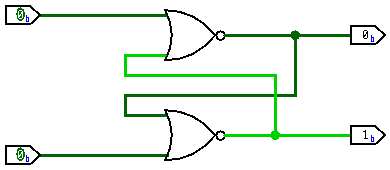
\includegraphics[width=\textwidth, center]{./figures/nor_rs_flip_flop_000.png}}
        \only<2>{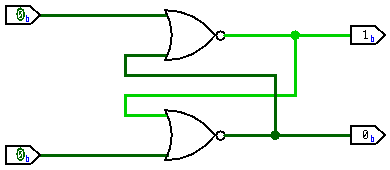
\includegraphics[width=\textwidth, center]{./figures/nor_rs_flip_flop_001.png}}
        \only<3>{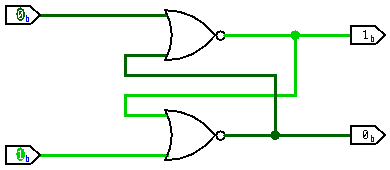
\includegraphics[width=\textwidth, center]{./figures/nor_rs_flip_flop_011.png}}
        \only<4>{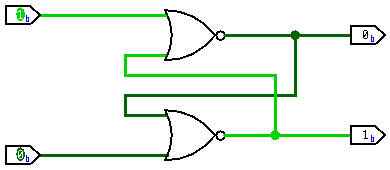
\includegraphics[width=\textwidth, center]{./figures/nor_rs_flip_flop_100.png}}
        \only<5>{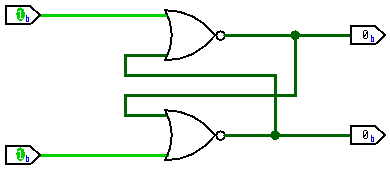
\includegraphics[width=\textwidth, center]{./figures/nor_rs_flip_flop_110.png}}
      \end{column}
    \end{columns}
  \end{solutionnoinc}
\end{frame}
\begin{frame}[allowframebreaks]{Aufgabe \thesection}{NOR RS-Flipflop}
  \stepcounter{exercise}
  \begin{solution}
    \begin{itemize}
      \item bei a = b = 0 wird der aktuelle \alert{Wert gehalten}
      \item bei a = 0, b = 1 wird c auf 1 und d auf 0 gesetzt 
      \item bei a = 1, b = 0 wird c auf 0 und d auf 1 gesetzt
    \end{itemize}
  \end{solution}
  \begin{solution}
    \begin{itemize}
      \item a und b sind \alert{active-high}, da sie durch das Heben auf 1 aktiviert werden
    \end{itemize}
  \end{solution}
  \begin{solution}
    \begin{itemize}
      \item die Belegung a = 1, b = 1 ergibt keinen Sinn, da 
      \begin{itemize}
        \item es bei gleichzeitigem Absenken von a und b zu \alert{Flackern} kommen kann
        \item da es für die diese Eingangsbelegung \alert{nur einen stabilen Zustand} gibt. Daher kann \alert{nur ein Wert \enquote{gespeichert}} werden
      \end{itemize}
    \end{itemize}
  \end{solution}
\end{frame}
